
\section{Introduction}

\subsection{Problem Definition}

A \emph{content item} is some unit of information, such as a statement, graph,
table, example, and so forth.  An educationl television program, interactive
tutorial or university lecture (generally, these may all be called programs)
can be broken down into these units of information.  Call an item $\chi$; then
the $i^{th}$ item to be seen is $\chi_i$, and the time at which it is seen
$t_i$.  Then $(\chi_i, t_i)$ represents the $i^{th}$ item and its scheduled
time.  

For that matter, any program can be thought of as a sequence of these tuples,
thereby forming a schedule of items: 

\begin{equations}
\label{eq:schedule}
   X = \langle (\chi_1, t_1), (\chi_2, t_2), \ldots (\chi_n, t_n) \rangle.
\end{equations}
\vspace{2pt}

Furthermore $\chi$ could be a question, which could be thought of as an item
which accepts a response back that has a correct answer.  Items and questions
share many similar properties which help to distinguish them, such as the
ones in Fig~\ref{fig:properties}.

The main question this body of work seeks to answer is this: \emph{based on
input from the student on any subset of questions in an item schedule, how
should the remaining questions be scheduled}?

\subsection{Novel Contributions}

The answer to this question required a series of novel contributions to the
fields of intelligent tutoring systems (ITS) and computer-aided assessment
(CAT).  Specifically:

\begin{itemize}

 \item The creation of a data structure in the form of a graph, whose nodes
 contain information relevant to the assessment process, and whose edges
 capture dependency relationships among questions;

 \item A modification to an existing assessment theory known as Item Response
 Theory, which however providing a mature means of assessing student ability,
 benefited from an account of dependency relationships;
 
 \item A scheduler, or algorithm whose purpose was to determine what the
 questions should be given the item parameters and the students' response
 sets;

 \item An addendum to an existing theory of memory, forgetting, and practice,
 which could then be integrated into the scheduler to provide a fuller-featured
 system.

\end{itemize}

In addition to this, the body of work rests upon other incidental novel
contributions, such as the separation of Bloom level and difficulty
\cite{castleberry}.

\section{Bloom's Taxonomy}

Bloom's cognitive taxonomy organizes questions into levels depending on the
cognitive functions required of the answerer.  The levels are: knowledge,
comprehension, application, analysis, evaluation, and synthesis.  A brief
overview is given in Table~\ref{tab:bloom}, with definitions and examples of
questions covering the concept of for-loops:

\begin{table}[!p]
\label{tab:bloom}
\caption{The levels of Bloom's taxonomy defined}
\vspace{12pt}
\begin{tabularx}{\textwidth}{||l|X|X||}
\hline \hline
\rowcolor{Gray}
Level &  Explanation & Example Question \\\hline
Knowledge & Recalling factual information.   
& {What is a for-loop?}
\\ \hline
Comprehension & Assigning meaning to information.   
& {What does the example for-loop output? (Give example.)}
\\ \hline
Application & Applying a rule to a specific instance.   
& {How can the update statement of the loop be changed to print 
only even numbers?}
\\ \hline
Analysis 
& Breaking information into parts and exploring relationships.   
& {What would happen if the update statement decremented instead of incremented the counter?}
\\ \hline
Evaluation 
& Judging the use of knowledge or the validity of an
argument.   
& {Which is better for reading user input: a for-loop or a
while-loop? Why?} 
\\ \hline
Synthesis 
& Utilizing knowledge to create a new solution to
satisfy a goal.   
& {Write a for-loop to print only even numbers up to ten.}
\\ \hline \hline 
\end{tabularx}
\vspace{36pt}
\end{table}

\begin{table}[!p]
\label{tab:grades}
\caption{Grades mapped to trait ability levels}
\vspace{12pt}
\begin{tabularx}{\textwidth}{||l|c|X||}
\hline\hline
\rowcolor{Gray}
Letter  & $\theta$  & Explanation \\\hline
F  & -3.0   & unsatisfactory \\\hline
D- & -2.5   &                \\
D  & -2.0   & minimal        \\
D+ & -1.5   &                \\\hline
C- & -1.0   &                \\
C  & -0.5   & acceptable     \\
C+ & 0.0    &                \\\hline
B- & 0.5    &                \\
B  & 1.0    & good           \\
B+ & 1.5    &                \\\hline
A- & 2.0    &                \\
A  & 2.5    & distinguished  \\
A+ & 3.0    &                \\\hline\hline
\end{tabularx}
\vspace{36pt}
\end{table}


Each category depends on the cognitive functions used in the previous category.
That is, comprehension requires knowledge, application requires comprehension,
and so forth.  Furthermore the mastery of one of the levels is with respect to
a given concept.  A student may be able to synthesize solutions to problems
dealing with expressions, but may not possess knowledge of equations, and thus
could not solve problems involving equations.

The utility of Bloom's taxonomy lies in its ability to pinpoint the underlying
cause of the student's problem-solving impasses \cite{shuhidan2011}.  
There is even evidence to suggest that Bloom levels correspond to different
electroencephalographic (EEG) signatures \cite{chatterjee2015}, implicating
distinct brain functions in their use. 

Suppose a test of mastery of loops is given with the comprehension question
``What does such-and-such loop output?'' is given, and the student reaches an
impasse.  If the question ``What are the three expressions of the loop and what
do they do?'' is asked and the student does not know, the impasse can be
attributed to a lack of knowledge about loops.  If the student does know about
the loop expressions but still cannot answer, one might instead attribute it to
a comprehension difficulty \emph{as such}; which might be remedied by giving
some examples to build intuition, then continuing to test at the comprehension
level.

Educators may have an intuitive notion of how to do this, but Bloom's taxonomy
gives the ability to examine the impact of questions scientifically.  By
identifying the tested concept and the Bloom level of exercises, one can then
form hypotheses about student responses to questions.  

\subsection{The Interpretation in Computer Science}

Bloom's taxonomy has been proven to be useful at the undergraduate level, and
particularly in the field of software engineering \cite{britto2015,
mahmood2014}.  It has seen success in program comprehension
\cite{buckley2003}, where the asking of comprehension questions fosters code
reading \cite{losada2008}. In addition, it has been useful for pinpointing the
difficulties of novice programmers in a guided learning approach
\cite{shuhidan2011}.  It been used to identify a marked preference for
higher-level problems for those able to solve them \cite{bruyn2011}
\cite{goel2004}.  At least two experiments have shown the effect of item
ordering on performance \cite{newman1988effect,castleberry2016effect}, and the
taxonomy has even been applied to create ratings of courses based on the
average Bloom levels of tasks and questions in the course
\cite{oliver2004course}.

In spite of all this, there is an ongoing debate regarding the applicability of
Bloom's taxonomy to computer science \cite{johnson2006bloom,
fuller2007developing, thompson2008bloom}.  The crux of this debate centers
around the interpretation of Bloom levels: not only how questions map to Bloom
levels, but also regarding the progression of Bloom levels over the span of a
course or curriculum.  

A tacit assumption in much of the research is that Bloom levels equate to
difficulty levels.  While there is certainly a relationship between Bloom level
and difficulty in the ``ordinary course'' of devising problems, a distinction
can be made between the two.
% TODO: (SRB) cite the papers you cite in the difficulty paper regarding this
% assumption.

\subsection{Assumptions of this Work}

% TODO: (SRB) cite the prior research. I know it's not published yet.
Prior research by the author supports the view that Bloom level and difficulty
are separable parameters of a content item.  This work will proceed on the
assumption to that effect. 

In addition, some of the components of this body of work, particularly those
pertaining to memory and recall, are supported by many decades of empirical
research \cite{ebbinghaus}.  While the study of intelligent tutoring systems
has seen attempts to validate addendums to these theories which accommodate
re-activation of forgotten knowledge, none have undergone extensive empirical
testing as is typical for psychological models.  The components of this body of
work regarding re-activation introduce hypotheses.

\section{Item Response Theory}

Here is introduced a mature assessment theory known as Item Response Theory, an
alternative to Classical Test Theory (CCT).  Whereas Classical Test Theory
assigns a student a grade based on the student's position in a distribution of
composite test scores, Item Response Theory accounts for item difficulty, item
discrimination, the probability of guessing the question correctly.

One of the main appeals of IRT is its incorporation of item difficulty.  As
will be shown later, this is pertinent to the interpretation of Bloom levels.  

According to Item Response Theory (IRT), in what is known as the 3PL or 3
parameter logistic model, the probability $p_i$ that a student answers
correctly the $i^{th}$ question on a test, is given by:

\begin{equations}
 \label{eq:irt}
  p_i(\theta_s) = \gamma_i + \frac{1-\gamma_i}{1+e^{\alpha_i(\theta-\beta_i)}}
\end{equations}

where:

\begin{itemize} 

 \item $\alpha$ is the item discrimination, or how well the item can
 distinguish students of varying trait ability;

 \item $\beta$ is the question difficulty, 

 \item $\gamma$ is the probability of guessing the answer correctly,

 \item and $\theta$ is the \emph{trait ability} of the student, or the
 student's particular ability to answer that question correctly.

\end{itemize} 

A graph of the IRT curve for the parameters $\alpha=1, \beta=0, \gamma=0$ is
shown \ref{fig:irt}.

\begin{figure}[p!]
 \label{fig:irt}
 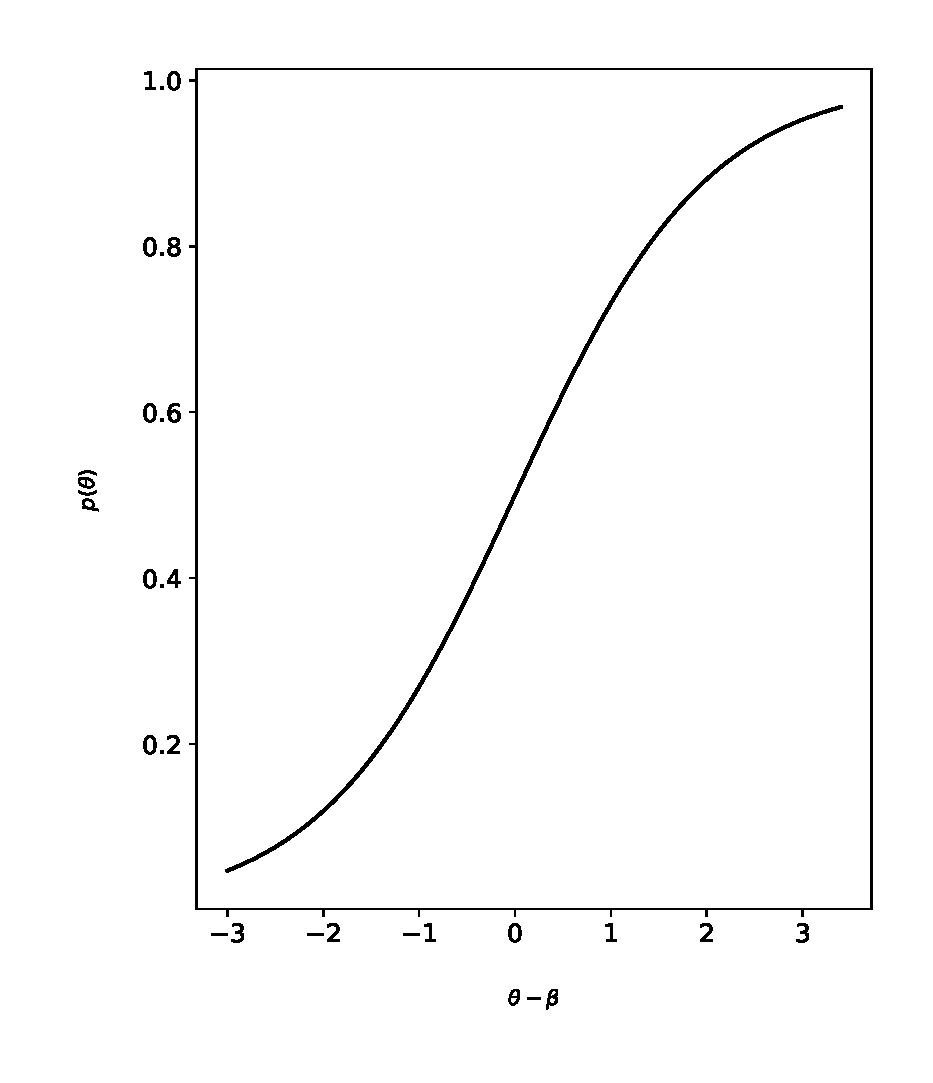
\includegraphics{fig/irt.eps} 
 \caption{A probability curve in Item Response Theory.}
\end{figure}

\begin{figure}[p!]
 \label{fig:mle}
 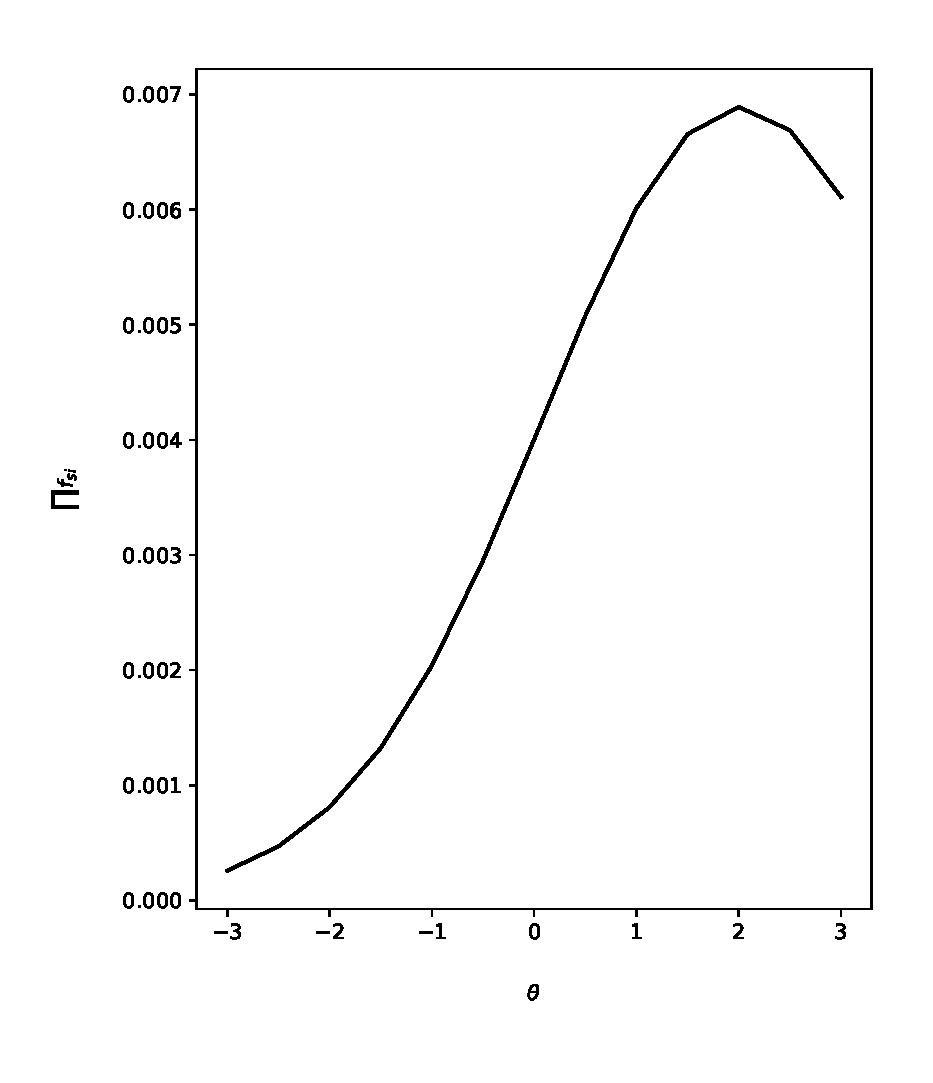
\includegraphics{fig/mle.eps} 
 \caption{A maximum-likelihood estimation for IRT}
\end{figure}

Note that $\alpha_i$, $\beta_i$, and $\gamma_i$ are parameters of the item $i$;
however $\theta_s$ is particular to the student $s$.  

The question difficulty $\beta$ can be estimated by the proportion of students
who pass the question.  The value $\beta$ is analogous to standard deviation in
classical test theory.  If a model of student ability based upon the number of
standard deviations from the mean is desired, and the scores are normally
distributed, then the $\beta$ values can simply be obtained from the
probability density function for a Student's t distribution.

Supposing $\phi$ is the proportion of students who pass the question, $f(v, x)$
is the probability density function for the Student's t-distribution with $v$
degrees of freedom then the relationship between $\phi$ and $\beta$ in such an
assignment would be given by

\begin{equation}
  \phi = \int_{\beta}^{\infty} f(v, x) \ dx
\end{equation}

That is, $\beta$ is the number of standard deviations such that the area from
$\beta$ to $\infty$ under the curve is equal to the proportion of students who
pass the question.  The value can also be obtained from a t-table.

Insofar as the intelligent tutoring system is concerned, the instructor or user
is free to assign $\beta$.  Varying assignments of the $\beta$ scores will
slightly alter the behavior of the system; if a given question is tagged as
easier (that is, assigned a lower $\beta$ value), it will have a greater chance
of appearing earlier in any given student's schedule.

If only $\beta$ is used as a parameter, the resulting model is known as the
1PL or 1 paramter logistic model:

\begin{equations}
 \label{eq:irt}
  p_i(\theta_s) = \frac{1}{1+e^{\theta-\beta_i}}
\end{equations}

\begin{figure}[p!]
 \label{fig:ctt}
 \includegraphics{fig/ctt.eps} 
 \caption{The standard normal curve; the distribution of test scores
  as modeled by Classical Test Theory}
\end{figure}

\begin{figure}[p!]
 \label{fig:pl1}
 \includegraphics{fig/pl1.eps} 
 \caption{The 1PL Item Response Theory model, where $\beta$=1}
\end{figure}


The item discrimination, $\alpha_i$, is defined as the Pearson product-moment
correlation coefficient between the item responses and the composite score on
the test.  Since the item responses are dichotomous, a correlation known as the
point-biserial correlation is computed.  It is defined as:

\begin{equations}
  \alpha_i = \frac{M_1 - M_0}{s_n} \sqrt{\frac{n_0 n_1}{n^2}}
\end{equations}

where $M_1$ is the mean composite score for all correct responses; $M_0$ is the
mean composite score for incorrect responses; $n_0$, $n_1$, and $n$ are number
of incorrect, correct, and total responses, respectively; and the standard
deviation $s_n$ is defined as:

\begin{equations}
  s_n = \sqrt{ \frac{1}{n} \displaystyle\sum_{i=1}^n (X_i - \overline{X})^2} 
\end{equations}

where $X_i$ is the ith response and $\overline{X}$ is the mean of the
responses.  $\alpha$ values have range $[-1, 1]$.  Positive values indicate
that the question is positively discriminating; it is a question which is
useful for gauging the constructs which the composite score seeks to measure.
Students who succeed on a question with a higher $\alpha$ are more likely to
have higher composite scores.  Likewise, negative values indicate that the
question is inversely related to composite score.  Values near zero indicate
that the question is unrelated.

If only $\alpha$ and $\beta$ are used as parameters, the resulting model is
known as the 2PL or 2 paramter logistic model:

\begin{equations}
 \label{eq:irt}
  p_i(\theta_s) = \frac{1}{1+e^{\alpha(\theta-\beta_i)}}
\end{equations}


The probability of guessing is defined as

\begin{equations}
  \gamma_i = \frac{1}{m_i}
\end{equations}

where $m_i$ is the number of options in a multiple choice question.  It is
assumed that each option is equally likely to be chosen if a student with
very low trait ability were to answer the question; that is, there can be
no allowance for logical process-of-elimination tactics.

Addition of the probability of guessing results in the 3PL model, given
in Eq~\ref{eq:irt}.

If the trait ability of the student is known in addition to the item
parameters, then the probability of a correct response can be calculated.
However, it is more often than not the case that the response set of the
student is known, and trait ability is unknown.  In such a case, a variety of
techniques are deployable.

\begin{figure}[p!]
 \label{fig:pl2}
 \includegraphics{fig/pl2.eps} 
 \caption{The 2PL Item Response Theory model, where the item discrimination 
 $\alpha=.5$ and $\beta=0$}
\end{figure}

\begin{figure}[p!]
 \label{fig:pl3}
 \includegraphics{fig/pl3.eps} 
 \caption{The PL3 Item Response Theory model, where $\alpha=1$ and $\beta=0$,
 and probability of guessing $\gamma=.25$}
\end{figure}

Trait ability in IRT can be obtained using a maximum likelihood estimation
(MLE) method, which finds a maximum-likelihood estimate of $\theta$ by testing
a range of $\theta$ values with the IRT formula \cite{baker2004}.  Later it
will be shown how $\theta$ can be estimated.  Another potential technique is
Newton-Raphson, which in most other applications would be the more efficient
and desirable method \cite{baker2004}.  It will later be discussed why the MLE
method is preferred.

%The utility of IRT is that it requires fewer questions to gauge trait ability
%due to its account of other factors ($\alpha, \beta, \gamma$). It is thus
%reputed to be a more mature means of assessment than CTT.

Until now, the fusion of IRT and Bloom's taxonomy has only existed in the
literature as a possibility \cite{sitthisak}.  This work seeks to reconcile
the two by offering a compatible interpretation of Bloom's taxonomy.
%TODO: (SRB) I don't think this is true. See email I sent you on 1/24/2017.

\subsection{Evaluation of Trait Ability}

Consider a set of content items or questions for which the answer is either
incorrect or correct.  This is true in the case of multiple choice questions
(as well as true-false, which is a subset of multiple-choice questions).

Suppose the student has a response set for content items: 

\begin{equations}
  \label{eq:responses}
  X_s = x_{s1}, x_{s2}, \ldots, x_{si}, \ldots x_{sn}
\end{equations}

Here $X_s$ is the response vector of student $s$, and $x_{si}$ is the
correctness of the response to content item $i$ by student $s$; it is zero if
the response is incorrect, or 1 if it is correct.  

These questions may be of various and sundry discriminations, difficulties, and
probabilities of guessing.  The first question may have $\alpha_1=.5$,
$\beta_1=1$, and $\gamma_1=.25$; the second may only differ in its difficulty,
for example $\beta_2=-1$.  However, it shall be assumed that the set of
content items for which the student has provided responses are for the same
concept and the same Bloom taxonomic level.  The reason for this assumption
will become apparent later.

Recall that the probability $p_{si}$ of student $s$ answering the $i^{th}$
question correctly is:

\begin{equations}
  p_{si}(\theta_s) = \gamma_i + \frac{1-\gamma_i}{1+e^{\alpha_i(\theta_s-\beta_i)}}
  \tag{\ref{eq:irt}}
\end{equations}

Since $\theta_s$ is unknown but the response set is known, one method for
determining $\theta_s$ is by guessing a range of possible values.  First, one
can define a function $f_{si}$:

\begin{equations}
f_{si}(\theta_s) =\left\{
         \begin{array}{ll}
               p_{si}(\theta_s) & \mathrm{if}\  x_{si} = 1 \\
               q_{si}(\theta_s) & \mathrm{otherwise}
         \end{array}
       \right.
\end{equations}
% TODO: (SRB) Do you mean p_{si} above when you type p_i?

where 

\begin{equations}
   q_{si}(\theta_s)  = 1 - p_{si}(\theta_s).
\end{equations}

That is, $f_{si}$ assumes the probability $p_{si}$ if answered correctly and
$q_{si}$ if not answered correctly.  Proceeding on the assumption that each of
the observations (that is, responses in the response set) is independent, the
probablity of observing a total response set given a particular $\theta_s$
value is the product of the probabilities $f_{si}$ for all $i$, $1 \leq i \leq
n$, or

\begin{equations}
  \prod_{i=1}^n f_{si}(\theta_s).
\end{equations}

Supposing that there exists some $\theta_s$ which maximizes this product,
the most likely value for the student's true trait ability $\theta_s$ is
defined by:

\begin{equations}
  \theta_s = 
  \underset{\theta}{\textrm{argmax}}
  \Bigg[ 
  \prod_{i=1}^n f_{si}(\theta).
  \Bigg]
\end{equations}


that is, that value of $\theta_s$ which maximizes the product which gives the
probability of all the observations occuring together, given $\theta$.  To
obtain this, products for a range of possible $\theta$ values are calculated.

In the intelligent tutoring system which has been constructed, there are only
thirteen such values, drawing from the +/- system.  The mapping of grades to
trait ability levels is given in Table~\ref{tab:grades}.  This mapping could
also be applied to difficulty levels of questions.  A ``C question'' is one
which students of average trait ability (and perhaps just more than half the
class) may be expected to answer; an ``A+ question'' is a very difficult
question which students of only A+ ability at the time of asking may be
expected to answer; and an ``F question'' is one which may be used to determine
if a student's trait ability is minimally satisfactory.  This mapping lends to
a intuitive understanding of trait ability--as the familiar letter grade.  An
MLE may thereby effectively grade the student.

% TODO: (SRB) Something should be said about the confidence in the trait
% ability assessment given above. In principle, a letter grade could be
% obtained from 2 questions.

To that end, rather than using a fine-grained MLE, it makes practical sense to
calculate products for these thirteen values of $\theta$, since higher
granularity than the +/- system is not useful for final grade assignment, nor
is necessarily more intuitive for the student or instructor.  Restricting the
products calculated to this set of values also makes sense from an efficiency
standpoint.  The total time complexity of the MLE is linear in the size of the
response set, regardless of the number of guesses in $\theta$; while not
asymptotically reduced from using a smaller step size, it is five times faster
than the typical choice of $10^{-1}$, and fifty times faster than the
fine-grained $10^{-2}$.  A graph calculating likelihoods for MLE is depicted in
Figure~\ref{fig:mle}.

% Talk about gradient descent and Newton-Raphson

The total number of MLE estimations for trait ability throughout a course is
equal to the total number of responses for all questions throughout a course,
which can be quite large; it is proportional to the number of students times
the number of items. 


\section{Previous Literature}

\subsection{Works Mentioning Bloom's Taxonomy and Item Response Theory}

There has been one suggestion by Sitthisak et al.  linking Item Response Theory
with Bloom's taxonomy which interprets Bloom levels as difficulty levels.  That
is, the values of $\beta$ from Item Response Theory are mapped directly to
Bloom levels \cite{sitthisak}.  This suggestion exists in the form of a
proposal to implement a computer-aided tester using Item Response Theory.

Another study identifies difficulty by levels of Bloom's taxonomic levels, and
evidently applies Item Response Theory to scoring of the same questions;
however it is unclear how the Bloom levels are mapped ot Item Response Theory
$\beta$ values, or whether or not the mentioned difficulties were hypothesized
or actual difficulties \cite{osborne2013grounded}.  

It is discussed in Sec~\ref{sec:reconciling} why it is desirable for the
current intelligent tutoring system to maintain difficulty and Bloom levels as
separate entities.

Ghulman et al. may be the closest to a full separation of Bloom's taxonomy and
difficulty, as well as establishing the connection between Bloom's taxonomy and
Item Response Theory, as it categorizes questions by Bloom level before
applying a Rasch model to score them \cite{ghulman2009modern}.  The Rasch model
is a model simpler in nature than Item Response Theory which uses one paramter
and is derived from the data set itself.

\subsection{Categories of Systems}

Conole and Warburton have developed a classification system for such
computer-aided testing tools.  Web-based systems \cite{wang2004web} fall under
networked systems, which in turn fall under computer-based assessment
utilities, which in turn falls under computer-assisted assessment
\cite{conole2005review}.  Conole and Warbuton identify that Bloom's taxonomy is
often used as an outcomes-based categorization tool for questions, and that
Classical Test Theory and Item Response Theory are the two main ways in which
computer-aided systems score questions; however these are mentioned in
isolation.

Bejar distinguishes between two types of systems: deficit assessment and error
analysis \cite{bejar1984educational}.  Deficit assessment is concerned with
finding where a student is lacking (such as in trait ability), and error
analysis with what steps in the problem-solving process the student is making
errors in.  This distinction is similar to Anderson's characterization-based
models versus process-based models in intelligent tutoring systems; where
characterization-based models attempt to create a representation of the
student's strengths, process-based models attempt to simulate the student's
problem-solving processes \cite{anderson}.  The current work would fall
squarely within the realm of Bejar's deficit assessment-type system, or
Anderson's characterization-based model.

\subsection{Memory and Forgetting}

Ebbinghaus is credited with having created one of the first mathematical
memories of rememberance and forgetting \cite{ebbinghaus}.  In particular, he
identified that recall drops off exponentially with time.  Empirical studies
since then have supported his original finding.

John Anderson developed a model for process-based learning which could provide
the foundation for an intelligent tutoring system \cite{anderson}.  He called
this Adaptive Control of Thought-Rational (ACT-R).  In ACT-R, there are goals,
akin to problem statements; and rules, or processes used to solve problems; and
finally facts, or knowledge utilized in the course of applying rules.  In this
regard, the structure of an ACT-R model resembles a logic program.  Anderson
also developed a memory model for ACT-R fact and rule recall loosely based on
Ebbinghaus' recall functions, as well as models of re-activation of knowledge
generalized from his own empirial research.  \cite{bacon2003assessing}


\subsection{Executability} 

Finally, some supplementary work on the executability component of the
intelligent tutoring system has been done \cite{castleberry2011}.  One
component of the intelligent tutoring system allows for arbitrary code to
execute before a question or item is displayed to the student.  This feature
was inspired by earlier work on what are known as executable papers.
Executable papers are academic publications residing inside of a virtual (or
other) machine which have editable codes on the front-end and compilers or
interpreters on the backend.  The front-end codes may be edited, then the
paper may be re-compiled so that results from the codes are substituted back
into the paper.  

This idea was originally intended for use with computational science codes, but
was adapted for statistics codes \cite{castleberry2013}.  It has been
integrated into the present work to allow for sophisticated random-number
generation, and for the nature of the questions and items to change in response
to the student or other contextual data.


\subsection{Reconciling Bloom's Taxonomy with Item Response Theory}
\label{sec:reconciling}

A popular interpretation of Bloom's cognitive levels is that they are
difficulty levels, and that these difficulty levels are fixed
\cite{newman1988effect,oliver2004course,lord2007moving,
johnson2006bloom,fuller2007developing}.  Knowledge is easy; synthesis is hard.
We will call this the Bloom-equals-difficulty hypothesis.

A creative interpretation of this hypothesis is that per-student difficulty can
be explained in terms of the demotion of Bloom levels.  The synthesis \emph{and
therefore difficult} questions, once the solution is obtained, are reduced to
knowledge \emph{and therefore easy} questions.  Certainly, this is one possible
scenario.  However, it does not explain a student's ability to answer
altogether distinct synthesis problems; this is to suggest students engage the
cognitive functions of synthesis, presumably as an effect of learning the use
of those functions.  To maintain that Bloom equals difficulty would either
require sustaining the view that students are able to pass the questions
because of a demotion of the cognitive functions required (which poses a rather
cynical view of cognition and of education); or else some notion of trait
ability--in particular one which offsets difficulty, allowing an increase in
the probability of passing the question.

The latter option takes the shape of a primeval form of Item Response Theory,
mapping Bloom levels to $\beta$.  This is highly convenient for the hypothesis
that Bloom equals difficulty, as it becomes agreeable to evaluation with Item
Response Theory.  Nontheless, there are still several issues with the
hypothesis.

Consider first that exposure to knowledge and knowledge questions causes an
increase in $\theta$, provided the student acquires the knowledge.  According
to Bloom's theory, this would increase the probability of answering
comprehension questions correctly.  This agrees with the theory.  However,
according to Item Response Theory, it would also increase the probability of
answering application questions correctly even if no comprehension-level
questions are asked.  In fact, it is theoretically possible to design tests
with sufficient numbers of knowledge questions to place, for any $\beta$,
$\theta-\beta$ much greater than zero--that is for example to say, asking a
sufficient number of knowledge questions should give the reasonable assurance
that application-level ability is high enough not to bother testing it.

As many educators will no doubt agree, this is not the case. Even if a student
scores exceptionally well on knowledge questions, it gives no such assurance
that the student will score similarly on application-level questions.  Even if
knowledge and application scores are found to be correlated, there may be an
additional underlying factor contributing to both scores (such as
intelligence).  The application level is \emph{qualitatively} different; hence
it needs to be tested in spite of the value of $\theta$.

Second, if the hypotheses is strictly true, then there can exist no
counterexample to the claim.  That is to say that there exists no problem on a
lower Bloom level which is more difficult than a problem on a higher Bloom
level.  To take an example, it would be mistaken to call an application problem
easier than any comprehension problem. 

Counterexmaples with intuitive appeal can be constructed.  Take for-loops for
example.  To ask a student to print out the result of a simple loop which
prints numbers 1 to 10 should present an easy enough task.  This is an
application of the many rules of for-loops, but which does not require creative
synthesis or critical thinking on the part of the student (hence it is an
application problem). 

Consider then asking the student to impose a flowchart over the same code,
including the initialization, condition and update statements and the body of
the loop, and to indicate the start and stop of the loop.  Suppose the student
has seen flowcharts over similar loops before.  This is a test of
comprehension--in particular, comprehension of the internal workings (the
control flow) of the loop.    

The application problem above requires only an intuitive comprehension of the
loop: ``\emph{It prints the sequence from 1 up to 10 in steps of 1}'', the
student may realize.  It demands only shallow comprehension and the rule to be
applied is simple.  In the comprehension problem, on the other hand, a higher
degree of precision in comprehension of the loop is demanded to solve the
problem.  The comprehension problem also depends on mastery of the knowledge,
comprehension, and application of flowchart symbols.  Regardless, explaining
the control flow of the loop in full detail is a more difficult undertaking
than simply printing its output. 

Likewise, it is possible to ask the student to synthesize a loop printing the
first ten powers of two, then ask a comparatively difficult analysis question
in the form of an obfuscated loop code.  Impasses in this situation may be
attributed to a lack of knowledge or comprehension of the constructs used in
the presented code.  In the synthesis problem, the student has the advantage of
using known syntax; it is a ``constructed-response'' type of question, rather
than a closed-form question \cite{kuechler2010performance}. 

Third, by Bloom's own admission, it is possible to skip levels for certain
concepts \cite{bloom1956}.  In this case, the ordinality of Bloom levels
breaks down.  A plausible example is given above.  It is possible to teach how
to obtain the numeric sequences printed by for-loops before covering in full
detail the control flow of the loop.  In that particular case, application of
the rule does not depend on comprehension of the code construct.

Alternative interpretations of Bloom levels distinguish between facility or
difficulty and complexity of a problem \cite{hill1981testing,
thompson2008bloom}.  In such interpreations, the cognitive complexity has an
orthogonal relationship to the item difficulty.  The problem with such
interpretations, however, is that they do not readily explain the moderate
correlation that does exist between mean performance and Bloom level
\cite{hill1981testing}.


